\documentclass[11pt, nonacm=true, language=french, language=english]{acmart}

%%%% PREAMBULE MAIN FILE %%%%

%%% INFORMATIONS %%%

% last update 04/2022

%%% CONDITIONNING %%%




\usepackage{ifthen}

% \newcommand\documentisfrench{}
\newcommand\fr[2]{\ifthenelse{\isundefined{\documentisfrench}}{#2}{#1}}

% \newcommand\documentisbeamer{}
\newcommand\ifbeamer[2]{\ifthenelse{\isundefined{\documentisbeamer}}{#2}{#1}}

% \newcommand\documentissansserif{}
\newcommand\sans[2]{\ifthenelse{\isundefined{\documentissansserif}}{#2}{#1}}

%%% FILES %%%

%%%% PREAMBULE PACKAGES FILE %%%%

%%% FONTS %%%
\usepackage[T1]{fontenc}
\usepackage[utf8]{inputenc}

\fr{
  \usepackage[french]{babel}
}{}

\usepackage{CJKutf8}            % chinese, japanese, corean
%\usepackage{numprint}          % pretty digits

%% fourrier
%\usepackage{fourier}
%\usepackage[scaled=0.875]{helvet}
%\usepackage{courier}

%% sans serif
\sans{
  \usepackage{cmbright}
  \renewcommand{\familydefault}{\sfdefault}
}{}



%%% MISE EN PAGE %%%
\ifbeamer{}{
  % \usepackage[a4paper]{geometry}
  % \geometry{hscale=0.7,vscale=0.8,centering}
}



%%% UTILITIES %%%
\usepackage{xcolor}         % couleur
\usepackage{xspace}         % espace automatique

\usepackage{xurl}           % Pour citer les adresses web
\usepackage{hyperref}       % Liens

\usepackage{stackengine}    % Empiler du texte

\usepackage[cache=false]{minted}         % inclusion de code

\usepackage{alltt}          % verbatim avec commandes

\usepackage{enumitem}       % listes



%%% TABLES %%%
\usepackage{multirow}       % fusion de ligne dans les tableaux
\usepackage{booktabs}       % Allows the use of \toprule, \midrule and \bottomrule in tables



%%% IMAGES %%%
\usepackage{graphicx} % inclusion des graphiques
\usepackage{wrapfig}  % Dessins dans le texte.

\usepackage{tikz}
\usetikzlibrary{cd}             % commutative diagrams via https://tikzcd.yichuanshen.de/
\usepackage[framemethod=TikZ]{mdframed}



%%% TREES %%%
\usepackage[linguistics]{forest}


\ifbeamer{
  %%%% PREAMBULE BEAMER FILE %%%%

% This template has been downloaded from:
% http://www.LaTeXTemplates.com

\mode<presentation> {

  % The Beamer class comes with a number of default slide themes
  % which change the colors and layouts of slides. Below this is a list
  % of all the themes, uncomment each in turn to see what they look like.

  % \usetheme{AnnArbor}
  % \usetheme{Antibes}
  % \usetheme{Bergen}
  % \usetheme{Berkeley}
  % \usetheme{Berlin}
  % \usetheme{Darmstadt}
  % \usetheme{Dresden}
  % \usetheme{Frankfurt}
  % \usetheme{Goettingen}
  % \usetheme{Hannover}
  % \usetheme{Ilmenau}
  % \usetheme{JuanLesPins}
  % \usetheme{Marburg}
  % \usetheme{Montpellier}
  % \usetheme{PaloAlto}
  % \usetheme{Pittsburgh}
  % \usetheme{Rochester}
  % \usetheme{Singapore}
  % \usetheme{Szeged}

  % \usetheme{default}       % rien (cadre carré)
  % \usetheme{Boadilla}      % bas3
  \usetheme{CambridgeUS}   % bas3 + haut2
  % \usetheme{Copenhagen}    % bas2
  % \usetheme{Luebeck}       % bas2 + haut2 (cadre/puces carré)
  % \usetheme{Madrid}        % = Boadilla
  % \usetheme{Malmoe}        % = Luebeck
  % \usetheme{Warsaw}        % bas2 + cardes ombre

  % As well as themes, the Beamer class has a number of color themes
  % for any slide theme. Uncomment each of these in turn to see how it
  % changes the colors of your current slide theme.

  % \usecolortheme{albatross}
  % \usecolortheme{beaver}
  % \usecolortheme{beetle}
  % \usecolortheme{crane}
  % \usecolortheme{dove}
  % \usecolortheme{fly}
  % \usecolortheme{lily}
  % \usecolortheme{orchid}
  % \usecolortheme{rose}
  % \usecolortheme{seagull}
  % \usecolortheme{whale}
  % \usecolortheme{wolverine}

  % \usecolortheme{dolphin}
  \usecolortheme{seahorse}

  % \setbeamertemplate{footline} % To remove the footer line in all slides uncomment this line
  % \setbeamertemplate{footline}[frame number] % To replace the footer line in all slides with a simple slide count uncomment this line

  % \setbeamertemplate{navigation symbols}{} % To remove the navigation symbols from the bottom of all slides uncomment this line

  % \setbeamercovered{transparent} % Fait apparaître les animations en grisé (utile pour la conception, mais peut être commenté lors de la remise du document final)

  % Pour utiliser une police à empattements partout
  % \usefonttheme{serif}

  % Pour rajouter la numérotation des frames dans les pieds de page
  % \newcommand*\oldmacro{}%
  % \let\oldmacro\insertshorttitle%
  % \renewcommand*\insertshorttitle{%
  % \oldmacro\hfill%
  % \insertframenumber\,/\,\inserttotalframenumber}


  % section/subsection
  \setbeamertemplate{section in toc}{%
    \quad ({\inserttocsectionnumber})~{\inserttocsection}%
  }
  \setbeamertemplate{subsection in toc}{%
    \quad\quad $\rhd$~{\inserttocsubsection} \\%
  }

  \setbeamertemplate{navigation symbols}{} % remove nav bar

}

% table des matieres (à paramétrer selon le document)
\setcounter{tocdepth}{2}

\newcommand\tocpage{
  \begin{frame}
    \tableofcontents[firstsection = 2 , currentsubsection]
  \end{frame}
}


%% arbres dans beamer (forest)
% permet d'utiliser onslide=<>{} pour animer les arbres (beamer)
\tikzset{onslide/.code args={<#1>#2}{
    \only<#1>{\pgfkeysalso{#2}}
  }}

\tikzset{
  invisible/.style={text opacity=0, draw opacity = 0},
  visible on/.style={alt=#1{}{invisible}},
  alt/.code args={<#1>#2#3}{%
    \alt<#1>{\pgfkeysalso{#2}}{\pgfkeysalso{#3}} % \pgfkeysalso doesn't change the path
  },
}
\forestset{
  visible on/.style={
    for tree={
      /tikz/visible on={#1},
      edge+={/tikz/visible on={#1}}}}}

}{}

%%%% PREAMBULE MACROS FILE %%%%


\PassOptionsToPackage{svgnames}{color}


% Espace automatique après un guillemet fermant
\fr{
  \renewcommand{\fg}{\fg\xspace}
}{}

%% parenthèses, crochets & accolades qui s'adaptent à la taille de ce qu'il y a à l'intérieur
\newcommand{\ap}[1]{\left(#1\right)}        % auto parenthesis
\newcommand{\ab}[1]{\left[#1\right]}        % auto bracket
\newcommand{\acb}[1]{\left\{#1\right\}}     % auto curly bracket


%% Puces pour les listes
\setitemize[1]{label=$\diamond$}
\setitemize[2]{label=$\circ$}
\setitemize[3]{label=$\star$}

\setenumerate[1]{label=\arabic*.}
\setenumerate[2]{label=\theenumi\arabic*.}
\setenumerate[3]{label=\theenumii\arabic*.}
\setenumerate[4]{label=\theenumiii\arabic*.}
% \setenumerate[2]{label=\alph*.}
% \setenumerate[3]{label=\roman*.}

% style d'item description
\renewcommand{\descriptionlabel}[1]{%
  \hspace\labelsep \upshape\bfseries \textit{#1}%
}


% point median
\newcommand\ptm\textperiodcentered

%soulignement
\newcommand\ul\underline


% panneau attention
\newcommand\danger{
    \makebox[1em]{
        \makebox[0pt][s]{
            % \raisebox{.1em}
            {\footnotesize !}
        }
        \makebox[0pt]{
          \raisebox{-0.1em}
          {\color{red}\Large$\bigtriangleup$}
        }
    }
}


%% écrire une remarque
\newcommand{\rk}[1]{$\rhd$ \textbf{Remar\fr{que}{k}} \emph{#1} }
\newcommand{\qrk}[1]{$\rhd$ \emph{#1} } % quick remark : pas de texte


% encadre le texte passe en parametre sur toute la largeur de la page
\newcommand{\longbox}[1]{
    \begin{center}\fbox{\parbox{\textwidth}{
        #1
    }}\end{center}
}


%% signatures
% manuscrite + nom dessous
\newcommand{\sign}
{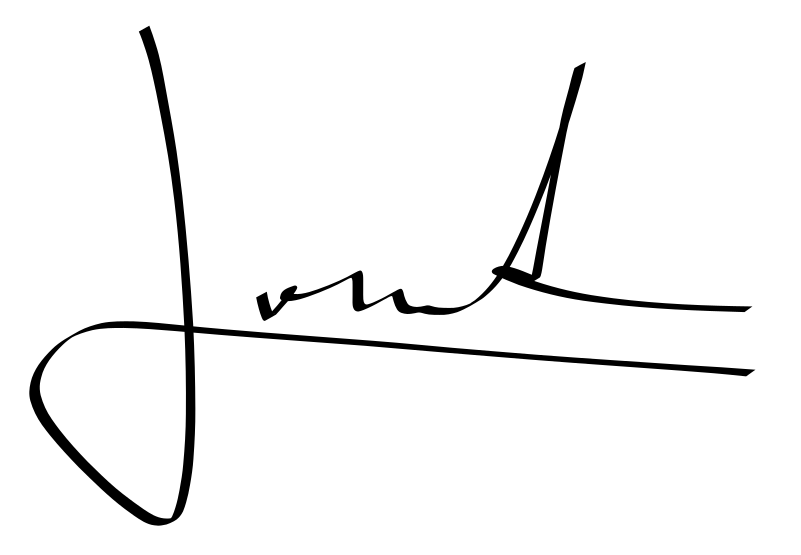
\includegraphics{preambule/signature_rj_small.png}\\ Robin \bsc{Jourde}}
% manuscrite + nom aligné à droite
\newcommand{\rsign}{\begin{flushright}\sign\end{flushright}}
% nom
\newcommand{\qsign}{Robin \bsc{Jourde}}
% nom aligné à droite
\newcommand{\rqsign}{\begin{flushright}\qsign\end{flushright}}



% email
\newcommand{\mailto}[1]{\href{mailto:#1}{\texttt{#1}}}


%%% PACKAGES %%%
\usepackage{amssymb}
\usepackage{amsmath}
\usepackage{mathrsfs}
\usepackage{amsfonts}

\usepackage{amsthm}         % theoremes et preuves
\usepackage{bussproofs}     % preuves en déduction nat et autres règles

\DeclareMathAlphabet{\varmathbb}{U}{bbold}{m}{n} % mathbb pour les chiffres


%%% LETTRES GRECQUES %%%
\renewcommand\phi{\varphi}
\renewcommand\epsilon{\varepsilon}



%%% MACROS %%%
%% Ensembles gras
\newcommand\N{\mathbb N}
\newcommand\Z{\mathbb Z}
\newcommand\D{\mathbb D}
\newcommand\Q{\mathbb Q}
\newcommand\R{\mathbb R}
\newcommand\C{\mathbb C}
\newcommand\K{\mathbb K}
\newcommand\F{\mathbb F}
\newcommand\E{\mathbb E}
\renewcommand\P{\mathbb P}


%% chiffres gras
\newcommand\zero{\varmathbb 0}
\newcommand\one{\varmathbb 1}
\newcommand\two{\varmathbb 2}



%% Autres ensembles
\newcommand\0{\varnothing}

\newcommand\M{\mathscr M}
\newcommand\MnR{\M_n(\R)}
\newcommand\MnC{\M_n(\C)}
\newcommand\MnK{\M_n(\K)}

\newcommand\B{\mathcal B}
\newcommand\Cl{\mathscr C}
\newcommand\Fn{\mathscr F}

\newcommand\Sfrak{\mathfrak S}



%% Opérateurs classiques
\DeclareMathOperator\id{id}
\DeclareMathOperator\Vect{Vect}
\DeclareMathOperator\card{card}
\DeclareMathOperator\rg{rg}
\DeclareMathOperator\im{im}
\DeclareMathOperator\colim{colim}

%% Catégories
\newcommand\Set{\mathbf{Set}}
\newcommand\Yo{\!\text{\begin{CJK}{UTF8}{min}よ\end{CJK}}}
\newcommand\op{{\,^\text{op}}}
\newcommand{\cattxt}[2]{#1\mathbf{\textbf{-}#2}}
\newcommand{\nlab}[1]{\href{https://ncatlab.org/nlab/show/#1}{[\fr{voir sur le}{see on} nlab]}}

\DeclareMathOperator\st{st}
\DeclareMathOperator\ob{ob}
\DeclareMathOperator\Ran{Ran}
\DeclareMathOperator\Lan{Lan}
\DeclareMathOperator\Kl{Kl}
\DeclareMathOperator\Hom{Hom}

%% Divers

% equivalent
\newcommand{\eq}[1]{\underset{#1}{\sim}}

% fleche de limite
\newcommand{\tend}[2]{\underset{#1 \to #2}{\longrightarrow}} 

% definition d'une fonction
\newcommand{\func}[4]{
    \ \begin{array}{|lll}
        #1 &\longrightarrow& #2 \\
        #3 &\longmapsto& #4
    \end{array}
}

%bijection
\newcommand\bij{\xrightarrow{\sim}}

%autres fleches
\newcommand{\xto}[1]{\xrightarrow{#1}}
\newcommand\too{\multimap}

\newcommand\from{\leftarrow}
\newcommand\mapsfrom{\mathrel{\reflectbox{\ensuremath{\mapsto}}}}

%d rond
\newcommand\drond{\partial}

% carre de fin de preuve
\renewcommand\qedsymbol{$\square$}
\newcommand\cqfd{\begin{flushright}\qedsymbol\end{flushright}}

%% Theoremes FR
\theoremstyle{plain}
\newtheorem{thm}{\fr{Théorème}{Theorem}}[section]
\newtheorem{lem}[thm]{Lemm\fr{e}{a}}
\newtheorem{cor}[thm]{Corolla\fr{ire}{ry}}
\newtheorem{prop}[thm]{Proposition}
\newtheorem{obj}{\fr{Objectif}{Goal}}


\theoremstyle{definition}
\newtheorem{ex}[thm]{Ex\fr{e}{a} mple}
\newtheorem{dfn}[thm]{D\fr{é}{e} finition}
\newtheorem{nota}[thm]{Notation}

\theoremstyle{remark}
\newtheorem{rem}[thm]{Remar\fr{que}{k}}

%% Disjonctions de cas
\newenvironment{disjonction}{\begin{enumerate}[label=\textbf{Cas\fr{e}{}  \arabic*.}]}{\end{enumerate}}


\usepackage{listings}

\usepackage{letltxmacro}
\newcommand*{\SavedLstInline}{}
\LetLtxMacro\SavedLstInline\lstinline
\DeclareRobustCommand*{\lstinline}{%
  \ifmmode
    \let\SavedBGroup\bgroup
    \def\bgroup{%
      \let\bgroup\SavedBGroup
      \hbox\bgroup
    }%
  \fi
  \SavedLstInline
}

\lstdefinelanguage{links}{
  morekeywords={sig,fun,case,switch,if,else,typename,effectname,do,handle,shallowhandle,lexhandle,var,fresh},
  morecomment=[l]{\#},
  commentstyle=\color{gray}
}
\lstset{
  basicstyle=\ttfamily\footnotesize,
  captionpos=b,
  numberstyle=\tiny\color{gray},
  numbers=left,
  breaklines
}
\lstset{language=links}
\lstMakeShortInline!

\setcopyright{none}

\author[R. Jourde]{Robin Jourde}
\affiliation{%
  \institution{École Normale Supérieure de Lyon}%
  \country{France}%
}
\email{Robin.Jourde@ens-lyon.fr}
\author{Supervised by Sam Lindley}
\email{Sam.Lindley@ed.ac.uk}
\author{Daniel Hillerström}
\email{Daniel.Hillerstrom@ed.ac.uk}
\affiliation{%
  \institution{The University of Edinburgh}%
  \country{United Kingdom}%
}

\renewcommand\shortauthors{Robin Jourde}


\title[M1 Intership Report]{M1 Internship Report : Effect Typing for Links}
\subtitle{2 May 2022 -- 22 July 2022, The University of Edinburgh}

\date{2 May 2022 -- 22 July 2022}

\begin{document}


\begin{abstract}
  This paper is the report of my internship at the School of Informatics of the University of Edinburgh with Sam Lindley and Daniel Hillerström from 2 May 2022 to 22 July 2022.
  Effect handlers are a language feature that is becoming more and more widespread. They allow the user to define and compose many functionalities from exceptions to concurrency and probabilistic programming.
  Links is an experimental tierless functional language for the web, mainly developed in the University of Edinburgh. Among its numerous features, Links supports effect handlers.
  The goal of my intership was to improve the effect typing system of Links, allowing aliases, avoiding pollution and allowing polymorphic operations.
\end{abstract}


\maketitle

\tableofcontents

\newpage

\section{Introduction}

TODO

\section{Links}

\begin{fquote}[Links website \cite{links-org}]
 Links is a functional programming language designed to make web programming easier.
\end{fquote}

Links \citep{} is a tierless functional programming language for the web developed at the University of Edinburgh. Typical web development involves the manipulation of several \emph{tiers} which means several, sometimes really different, programming languages :
\begin{itemize}
  \item the server side written in Python or Java for instance
  \item the client side in JavaScript and HTML/CSS
  \item the database queries in SQL
\end{itemize}
This is neither elegant nor really practical and prevents easy binding between different parts of the program that need to communicate data. It can cause \emph{impedance mismatch}, ie situations where the objects required by the server do not match what the database provide and vice versa.

Links avoids these by providing the programmer one single language for each tier (HTML/CSS are still needed) that is compiled into bytecode for the server, JavaScript for the client and SQL for the queries.

Links also supports numerous useful features including
\begin{itemize}
  \item polymorphic variants
  \item regular expressions
  \item session types
  \item row typing
  \item effect handlers (see \ref{sec:handlers})
\end{itemize}
It is used as an experimental language by researchers to try out new ideas and what could be future widespread programming languages features.

Links is strict, statically typed and use a Hindley-Milner type system as well as a Rémy style row typing system \ref{sec:row-typ} \citep{row-typ}. Its syntax is inspired from JavaScript and ML. Its compiler \citep{} is written in OCaml.

\begin{rem}
  In appendix \ref{sec:tech}, the reader could find some technical points on Links syntax and semantics that are not worth it to develop here. He is invited to look at it whenever needed.
\end{rem}

\section{Effect handlers}
\label{sec:handlers}

In functional programming, functions are seen as black boxes that takes an input and computes an output. Though this view of \emph{pure} functions is convenient and pleases $\lambda$-calculus fans, it fails to accurately represent what real programming is. Computations interact with the outer world by many means :
\begin{itemize}
  \item input/output
  \item concurrency
  \item exceptions
  \item choice and non determinism
  \item ...
\end{itemize}
The ``outer world'' here stand for anything that is not the pure computation, from memory, other threads and user interaction to the evaluation context itself.
These interactions not taken into account by the black-box model are called \emph{effects}.

Gordon Plotkin and Matija Pretnar \citep{plotkin-pretnar} introduced a construct that allow \emph{composable} and \emph{customisable} user-defined interpretation of effects : \emph{effect handlers}. They give the programmer direct access to the context, in the form of a first class continuation, often called \emph{resumption}.

Effect handlers can be seen as a generalisation of exception handlers. One can perform an effect in the same way as one could raise an exception and this will transfer the flow control to a handler. It is given the delimited continuation between the point where the effect is performed and where it is handled and can use it
\begin{description}
  \item[0 times] and act as an exception handler
  \item[once] (linear handler)
  \item[twice or more] (non-linear handler) to simulate a choice for instance
\end{description}

Effect handlers are being shown a growing industrial interest nowadays. Below are listed some of the biggest projects that uses and implement some kind of effect handlers
\begin{itemize}
  \item GitHub code analysis library Semantic (used in more than 25 million repositories)
  \item Meta JavaScript UI library React (used in mire than 2 million websites)
  \item Uber Pyro language
  \item WebAssembly
\end{itemize}

TODO : refs ?

\subsection{Syntax and usage}

We give the Links syntax alongside with usage of effect handlers and operations. All examples in this report are written in Links.

Inside any segment of code, one can invoke an operation !Op! with payload !p! writing !do Op(p)!. This has to be scoped into a handler of this operation. It will take the payload and the resumption and decide what to do.

\begin{lstlisting}[caption=Handler,label=lst:handler]
  handle ( code ) {
    case <Op(p) => r> -> ...
    case x -> ...
  }
\end{lstlisting}

Listing \ref{lst:handler} give the syntax for a handler for !Op!, !code! being the code that can perform the operation. When the operation is invoked, the right hand side of line 2 is executed with !p! the payload and !r! the resumption bound in context. When !code! returns a value, line 3 is executed with !x! bound to that value.

If the handler gives the resumption a value !v!, it acts as if !do Op(p)! returned the value !v!. If the payload has type !t! and !v! has type !t'!, we say that !Op! has type !t => t'!.

The type system keeps track of what effects can be performed. A function from type !a! to !b! which can performs operations !Op1: t1 => t1'!, \dots, !Opk:tk => tk'! will have type !(a) {Op1:t1 => t1', ..., Opk:tk => tk'}-> b!.


\subsection{Examples}

\subsubsection{A first exception handler}
\label{sec:first-except-handl}

~

\begin{lstlisting}[caption=Fail invocation]
  sig assert_positive : (Int) {Fail:() => Zero|_}-> Int
  fun assert_positive(x) {
    if (x>0) x else absurd(do Fail)
  }
\end{lstlisting}

This first example shows a function !assert_positive! that takes an integer and returns it only if it positive, else, it raises the effect !Fail! (for details on !absurd! and the !Zero! type, see \ref{sec:tech:zero}). This is the simplest example when one operation is invoked with no payload.

\begin{lstlisting}[caption=maybe handler, label=lst:mb-h]
  sig maybe : (() {Fail:() => Zero|e}~> a) -> () {Fail{_}|e}~> Maybe(a)
  fun maybe(m) () {
    handle(m()) {
      case <Fail> -> Nothing
      case x -> Just(x)
    }
  }
\end{lstlisting}

This operation can be handled by handler \ref{lst:mb-h}. This is actually an exception handler since the resumption is not used in the right hand side (and thus can be omitted in the left hand side). The \emph{effect signature} is !{Fail: () => Zero}!, that means there is only one operation called !Fail! that will be handled.

When the operation !Fail! is invoked, the handler directly returns a value, here !Nothing!. When the computation returns a value, the handler will return that value, embedded in the !Maybe! type (on !Maybe! type, see \ref{sec:tech:maybe}).

The function !maybe! will take a computation that can perform the effect !{Fail: () => Zero|e}! ie the operation !Fail! and possibly other effects, captured by the row variable !e!, and returns something of type !a!. It will execute this computation, performing effects from !e! that should be handled by another handler at some point. In the end, it returns a value of type !Maybe(a)!.

The !Fail{_}! in the effect row indicates a polymorphic presence for the operation. Roughly it means that the operation can or cannot be present after. This is needed since the effect type system enforces that all operations in a row are distinct. !Fail! cannot belong to !e! because of the effect row of the input computation.

\begin{lstlisting}
  sig h2g2 : () {Fail:() => Zero|_}-> Int
  fun h2g2 () {
    assert_positive( -6 * -7 )
  }
  sig h2g2' : () {Fail:() => Zero|_}-> Int
  fun h2g2' () {
    assert_positive( -6 ) * -7
  }
\end{lstlisting}

We can then use the !maybe! function to handle the failures in functions !h2g2! and !h2g2'! :

\begin{lstlisting}[caption=Links console]
  links> maybe ( h2g2 ) () ;
  Just(42) : Maybe (Int)
  links> maybe ( h2g2' ) () ;
  Nothing : Maybe (Int)
\end{lstlisting}


\subsubsection{Drunk coin tossing}

We consider now a new operation !Choose! that can produce a boolean and use it to simulate a drunk coin toss. The drunk tosses the coin and either let it fall or catch it and see heads or tail.

\begin{lstlisting}[caption=Drunk toss]
  typename Toss = [| Heads | Tail |] ;

  sig toss : () {Choose:Bool|_}-> Toss
  fun toss () {
    if (do Choose) Heads else Tail
  }

  sig drunkToss : () {Choose:Bool, Fail:Zero|_}-> Toss
  fun drunkToss () {
    if (do Choose)
      # catch
      toss ()
    else
      # fall
      absurd(do Fail)
  }

  sig drunkTosses : (Int) -> Comp([Toss], {Choose:Bool, Fail:Zero|_})
  fun drunkTosses (n) () {
    if (n<=0)
      []
    else
      drunkToss() :: drunkTosses (n-1) ()
  }
\end{lstlisting}

We can define several handlers for this operation.

\begin{lstlisting}[caption=Toss handlers]
  # linear handler : always true
  sig h_true : (Comp(a,{Choose:Bool|e})) -> Comp(a,{Choose{_}|e})
  fun h_true (m) () {
    handle (m()) {
        case <Choose => r> -> r(true)
    }
  }

  # non-linear handler : all choices in a list
  sig h_all : (Comp(a,{Choose:Bool|e})) -> Comp([a],{Choose{_}|e})
  fun h_all (m) () {
    handle (m()) {
        case <Choose => r> -> r(true) ++ r(false)
        case x -> [x]
    }
  }
\end{lstlisting}

And then we can compose the different handlers in several ways.

\begin{lstlisting}
  links> maybe ( h_true ( drunkTosses(2) ) ) () ;
  Just([Heads, Heads]) : Maybe ([Toss])
  links> h_true ( maybe ( drunkTosses(2) ) ) () ;
  Just([Heads, Heads]) : Maybe ([Toss])

  links> maybe ( h_all ( drunkTosses(2) ) ) () ;
  Nothing : Maybe ([[Toss]])
  links> h_all ( maybe ( drunkTosses(2) ) ) () ;
  [Just([Heads, Heads]), Just([Heads, Tail]), Nothing, Just([Tail, Heads]), Just([Tail, Tail]), Nothing, Nothing] : [Maybe ([Toss])]
\end{lstlisting}

We try different combinations for 2 coin tosses. In the two first cases, there is no failure so the order of handlers won't matter. The coin is always catch and always on heads.

In the third case, !h_all! imposes that all possibilities are explored so at some point, the coin will fall. This causes a failure, catch by !maybe! that simply returns !Nothing!.

The last case is the most complicated one. The failures are catch by !maybe! \emph{under} !h_all!. That means !h_all! won't see failures and will take each result, whether it is a !Nothing! or a list of heads/tail and form its big list of all possibilities.


\subsection{Semantics}
\label{sec:semantics}

We give the operational semantics for handlers.
\[
  \begin{array}{rcl}
    !handle ( !v! ) { !H! }! & \longrightarrow & N[v/!x!] \\
    !handle ( !\mathcal E[!do !Op_{i}!( !v! )!]! ) { !H! }! & \longrightarrow & N_{i}[v/!p!, !fun (x)  { handle ( !\mathcal E[!x!] ! ) { !H! } }!/!r!] \\
                                                                             && Op_{i} \notin \mathcal E\\
  \end{array}
\]

where $H =
\left\{\begin{array}{l}
  !case x! \mapsto N \\
  !case ! \langle Op_{i}(!p!) \To !r!\rangle \mapsto N_{i} \\
  \dots \\
\end{array}\right.$

and $\mathcal E$ is an evaluation context : $\mathcal E ::= [] \mid !handle ( !\mathcal E! ) { !H! } ! \mid !var x = ! \mathcal E ! ; ! N$.

$Op \in \mathcal E$ means there is a handler for $Op$ in $\mathcal E$.

If there is a value $v$ inside the handler, we call the return case $N$ with !x! bound to $v$. When the handler is the most inner one that can handle the operation $Op_{i}$ invoke with some payload $v$, what is insured by $Op_{i}\notin \mathcal E$, we bind the payload and build the resumption before calling the case $N_{i}$.

The resumption is embedded in the current handler since operation $Op_{i}$ could be invoked in the rest of the evaluation context $\mathcal E$. This is called a \emph{deep} handler.

\paragraph{Shallow handlers}
Links also support \emph{shallow} handlers, ie handlers that do not automatically reuse the handler in the resumption. The programmer has to write it and can choose another handler if needed. Below is the new rule for shallow handler.
\[
  \begin{array}{rcll}
    !shallowhandle ( !\mathcal E[!do !Op_{i}!( !v! )!]! ) { !H! }! & \longrightarrow & N_{i}[v/!p!, !fun (x)  { ! E[!x!] ! }!/!r!] & Op_{i} \notin \mathcal E\\
  \end{array}
\]

\paragraph{Parameterised handlers}

Another useful feature of handlers is that they could be parameterised. The programmer can give the handler a parameter that is carried along the computation.

\begin{lstlisting}[caption=Example of parameterised handler]
  sig h_state : (a) -> (Comp(b,{ Get:()=>a, Put:(a)=>() | e })) ~> Comp((b,a), { Get{_}, Put{_} | e })
  fun h_state (init) (m) () {
    handle (m()) (s <- init) {
      case x -> (x, s)
      case <Get => r> -> r (s, s)
      case <Put(s') => r> -> r ((), s')
    }
  }
\end{lstlisting}

\begin{lstlisting}
  fun ex () {
    var x = do Get * 10 ;
    var x = 2*x + do Get ;
    do Put(x) ;
    ()
  }

  links> h_state (2) (ex) () ;
  ((), 42) : ((), Int)
\end{lstlisting}

A second parameter is given to the !handle! construct that binds a variable and the resumption will take an additional parameter.

In the example above, we use that feature to write a state-cell handler. There are two operations !Put! and !Get! that respectively write into the cell and read what is inside. The parameter here is just the content of the cell.

Here are the reduction rules for parameterised handlers
\[
  \begin{array}{rcll}
    !handle ( !v! ) ( s!\from w! ) { !H! }! & \longrightarrow & N[v/!x!, w/!s!] \\
    !handle ( !\mathcal E[!do !Op_{i}!( !v! )!]! ) !  & \longrightarrow & N_{i}[v/!p!, w/!s!, \\
    ! ( s!\from w! ) { !H! }!                        &                 & !fun (x, s')  { handle ( !\mathcal E[!x!] ! ) ( s!\from!s' ) { !H! } }!/!r!] \\
                                                     &                 & Op_{i} \notin \mathcal E\\
  \end{array}
\]

\begin{rem}
  A parameterised has to be deep since the parameter needs a handler to carry it.
\end{rem}

\paragraph{Relationships between handlers}

Those three kinds of handlers are equivalent in the sense that it is possible to express each of them using one other.

If it is easy to see how to express a deep handler from a parameterised handler or from a shallow handler, the converse is not so obvious. See \citep{ehgc}, section 4 or \citep{daniel-thesis}, section 6.

\section{Typing}

Links is a strongly statically typed language. In this section, we describe some main features of Links type system that allow us to type effect handlers.

\subsection{Rows}
\label{sec:row-typ}

In order to type effects, we store in function types the effects that are \emph{allowed} to be perform during the execution of that function. To do so we use rows. They are an unordered and labeled data and type structure. They are also used in others features of Links as records and variants.

In the most general setting, a row is defined by
\[
  R ::= \bullet \mid \rho \mid l:\delta;R
\]
where $\rho$ is a row variable, $l$ is a label and $\delta$ is a data. $\bullet$ denotes the empty row.

A row is said to be \emph{open} if it ends with a row variable and \emph{closed} if it ends with the empty row.

For actual records, the data are actual values of the language but in the typing setting (typing effects, records and variants), $\delta$ will be a presence (see \ref{sec:links-typ}).

We require also that in one row, labels are all distinct and we consider row equal up to reordering of pairs labels/data.

\begin{ex}
  $Fail:Zero; Choose:Bool; \bullet$ is a valid row and is equal to $Choose:Bool; Fail:Zero; \bullet$ but $Fail:Zero; Fail:Int; e$ and $Fail:Zero; Fail:Zero; e$ are not valid. In the open row $Choose:Bool; e$, $e$ could not be substituted by anything with label $Choose$.
\end{ex}


\subsection{Links Type System}
\label{sec:links-typ}

We describe in this section and the following Links type system. In order to avoid useless complexity, we focus on the parts of the type system that are useful to understand effect typing. We omit easy and common parts as well as some parts used only for other Links features.

Below is the type and kind syntax.

\[
  \begin{array}{lrrll}
    \text{Kinds}           & K & ::= & Type \mid Row \mid Presence & \\
                           &&\mid & \kappa & \text{kind variable} \\

    \text{Rows}            & R, E & ::= & \bullet & \\
                           &&\mid & l:P;R & \\
                           &&\mid & \rho & \text{row variable} \\

    \text{Presence}        & P & ::= & - & \text{absent} \\
                           &&\mid & T & \text{present with a type} \\
                           &&\mid & \theta & \text{presence variable} \\

    \text{Types}           & T, A, B & ::=\ & P & \text{primitive type} \\
                           &&\mid & T \to_{E} T & \text{function type} \\
                           &&\mid & T \To T & \text{operation type} \\
                           &&\mid & (R) & \text{record type} \\
                           &&\mid & [R] & \text{variant type} \\
                           &&\mid & \forall \alpha :: K. T & \text{polymorphic type} \\
                           &&\mid & A\ B & \text{type application} \\
                           &&\mid & \alpha & \text{type variable} \\

    \text{Primitive types} & P & ::= & Int \mid Bool \mid String \mid \dots &
  \end{array}
\]

We have three different kinds that are usual \emph{types}, \emph{rows} and \emph{presence types}.

Any label that appears into a row is associated with a presence type that indicates if the label is present in this row. If it is, we have to provide a type, otherwise this is not necessary and we just indicate the absence. One may wonder why are presence useful. After all, to know if a label is present into a row, looking at the row should be enough. This is true for closed rows but not for open ones. Writing $l:-;\rho$ implies that the row variable $\rho$ cannot stands for a row containing $l$ since a label cannot appear twice into a row. Absence guaranties that whatever the row variable is substituted with, this label will never occur.

\begin{rem}
  In \emph{closed} rows, absence is redundant :
  $$ l_{0}:- ; l_{1}:P_{1} ; \dots ; l_{k}:P_{k} ; \bullet = l_{1}:P_{1} ; \dots ; l_{k} : P_{k} ; \bullet $$
\end{rem}

\paragraph{Links syntax for presence and effect rows}
In Links, we write effect rows between braces !{ ... }!. For a label !A!, the absence is denoted !A-!, the typed presence !A:type! and the polymorphic presence !A{p}!, with !p! a variable of presence kind. The empty row is denoted by !{}!, the closed row $l_{1}:\delta_{1}; \dots; l_{k}:\delta_{k}$ is denoted by !{l1:d1, ..., lk:dk}! and the open row $l_{1}:\delta_{1}; \dots; l_{k}:\delta_{k}; e$ is denoted by !{l1:d1, ..., lk:dk | e}!.

\subsection{Typing handlers}
\label{sec:typing-handlers}

The typing judgment has to take into account the current allowed effects. We gather them into a row $R$ and we write $\Delta;\Gamma \vdash e : T / R$ for expression $e$ has type $T$ in context $\Delta;\Gamma$ and can perform effects in $R$.

\begin{rem}
  The context contains two parts $\Gamma$ and $\Delta$. $\Gamma = x : A ; \dots$ contains typed term variables and $\Delta = \alpha :: K; \dots$ kinded type variables.
\end{rem}

We give below the main typing rules that allow to understand how effect handlers should be typed. The other rules are the obvious ones and can be found in appendix \ref{sec:typing-rules}. For the sake of clarity, shallow and parameterised handlers rules have also been moved to the appendix.

\begin{prooftree}
  \AxiomC{$\Delta;\Gamma \vdash p : B / R$}
  \AxiomC{$R = l : B \To A ; R'$}
  \RightLabel{$Op$}
  \BinaryInfC{$\Delta;\Gamma \vdash do\ l(p) : A / R$}
\end{prooftree}

\begin{prooftree}
  \AxiomC{$\Delta;\Gamma \vdash f : B \to_{R} A / R$}
  \AxiomC{$\Delta;\Gamma \vdash t : B / R$}
  \RightLabel{$App$}
  \BinaryInfC{$\Delta;\Gamma \vdash f t : A / R$}
\end{prooftree}

\begin{prooftree}
  \AxiomC{$\Delta;\Gamma, x:B \vdash e : A / R$}
  \RightLabel{$Fun$}
  \UnaryInfC{$\Delta;\Gamma \vdash fun (x) \{ e \} : B \to_{R} A / R$}
\end{prooftree}

\begin{prooftree}
  \AxiomC{$\Delta;\Gamma \vdash m : B / R'$}
  \AxiomC{$\Delta;\Gamma, x:B \vdash n : A / R$}
  \AxiomC{$R' = l_{i} : B_{i} \To A_{i} ; R_{0}$}
  \AxiomC{$R = l_{i} : \theta ; R_{0}$}
  \noLine
  \BinaryInfC{$\Delta;\Gamma, p_{i}:B_{i}, r_{i}:A_{i} \to_{R} A \vdash n_{i} : A / R$}
  \RightLabel{$Handle$}
  \TrinaryInfC{$\Delta;\Gamma \vdash handle (m) \{ case\ x \mapsto n\ case \langle l_{i} (p_{i}) \To r_{i} \rangle \mapsto n_{i}\} : A / R$}
\end{prooftree}

\begin{prooftree}
  \AxiomC{$\Delta;\Gamma \vdash e : A / R$}
  \AxiomC{$R \subseteq R'$}
  \RightLabel{$WeakEff$}
  \BinaryInfC{$\Delta;\Gamma \vdash e : A / R'$}
\end{prooftree}

where $R \subseteq R'$ is defined by
\begin{table}[h!]
  \centering
  \begin{tabular}{ccccc}
    \AxiomC{}
    \UnaryInfC{$R \subseteq R$}
    \DisplayProof
    &
      \AxiomC{}
      \UnaryInfC{$R \subseteq \rho$}
      \DisplayProof
    &
      \AxiomC{$R \subseteq R'$}
      \UnaryInfC{$R \subseteq l:P;R'$}
      \DisplayProof
    &
      \AxiomC{$R \subseteq R'$}
      \UnaryInfC{$l:P;R \subseteq l:P;R'$}
      \DisplayProof
    &
      \AxiomC{$R \subseteq R'$}
      \UnaryInfC{$l:\theta;R \subseteq l:P;R'$}
      \DisplayProof
  \end{tabular}
\end{table}

Rule $Op$ states that invoking an operation requires a ambient effect row that contains it with the correct types. Rule $App$ ensure that, when applying a function, its effect row is compatible with the ambient one. The $Handle$ rule types a !handle! construct. The important thing to notice is that the row used to type $m$ obviously contains the operations $l_{i}$ handled and that after handling, all $l_{i}$s have been removed from the row. The last rule mentioned here ensures that the ambient effect row mentions effects that are \emph{allowed} to be performed but not necessary since an effect can be added to the row.

We say that an expression $e$ type-checks only if no unhandled effects are allowed : $\Delta;\Gamma \vdash e : T / \bullet$, noted $\Delta;\Gamma \vdash e : T$.


\begin{thm}
  If $\Delta;\Gamma \vdash e : T / R$, in the execution of $e$ only effects in $R$ are performed and not handled.
\end{thm}
\begin{cor}
  If $\Delta;\Gamma \vdash e : T$, in the execution of $e$ all effects are handled.
\end{cor}

See \citep{} for the proof.


\subsection{Polymorphism} TODO

\subsection{Bidirectional Typing} TODO ?


\section{Contributions}

During my internship I added some new features to Links that have been merged into the 0.0.0 release.

\subsection{Effect Aliases}

In Links we can define type aliases using the keyword !typename!.
\begin{lstlisting}[caption=Type alias examples]
  # sum type via variants
  typename BinTree(a) = [| Node(BinTree(a), a, BinTree(a)) | Leaf |] ;
  # product type
  typename IntPair = (Int, Int) ;
  # record type
  typename Pet = (name:String, age:Int, species:String, Fur:Bool) ;
  # function type
  typename Comp(a, e::Row) = () ~e~> a ;
\end{lstlisting}

But until now, there was no way to define such thing for effects. This is really usefull since when working with effects, the same set of effects show up everywhere.

Using the new keyword !effectname! we can now write an alias for an effect row :
\begin{lstlisting}
  effectname MyEffectRow(a, ... ,e::Eff, ...) = { Op1 : type, ... | e } ; # open row
  effectname MyEffectRow(a, ... ) = { Op1 : type, ... } ; # closed row
\end{lstlisting}

To use it in a signature or in another type or effect alias just apply it with the right arguments as for typename things. In arrows, it can be used as row variables:
\begin{lstlisting}
  () -MyEffectRow(args)-> ()
\end{lstlisting}

However, due to lack of kind inference, row variables and aliases have to be used carefully so that Links does not think they are of kind type. We need to write them most of the time between braces !{ | ... }!. For instance, if there is !effectname E(a::Eff) = {X : ... | a }! and a row variable !e::Eff!, you will have to write !E({ |e})!, and similarly for another effect alias instead of the variable. This makes the usage of several nested aliases a bit messy, it would be nice if it could be avoided.

Recursive effect aliases are not available for now. The aliases are replaced by the row they correspond to, aliases are not kept are not printed out.

The implementation is mostly inspired by what is done for type aliases.

\subsection{Fresh Labels}
\label{sec:fresh-labels}

\subsubsection{The pollution problem}
\label{sec:pollution-problem}

TODO + cf ref 44 Tes

We first introduce a problem that arises when playing with numerous effects and that we will be calling \emph{effect pollution}. Let us start with an example.

\begin{lstlisting}
  sig safe_sqrt : ( Comp(a, {Fail:Zero, Sqrt:(Float)=>Float| e}) ) -> Comp(a , {Fail:Zero, Sqrt{_} | e})
  fun safe_sqrt (m) () {
    handle (m())  {
        case <Sqrt(x) => r> -> r (if (x<0.0) absurd(do Fail) else sqrt(x))
        case x -> x
    }
  }

  sig maybe_sqrt : ( Comp(a, {Fail:Zero, Sqrt:(Float)=>Float| e}) ) -> Comp(Maybe(a) , {Fail{_}, Sqrt{_} | e})
  fun maybe_sqrt (m) {
    maybe ( safe_sqrt( m ) )
  }
\end{lstlisting}

Let !safe_sqrt! be a handler for the operation !Sqrt! that takes a float and computes its square root. If the number is negative, the handler raises a failure via the !Fail! operation. Let !maybe_sqrt! the composition of the !maybe! handler for failures seen previously and the !safe_sqrt! handler.
\begin{lstlisting}
  fun shrink (x) {
    var y = do Sqrt(x) ;
    if (y < x)
      y
    else
      absurd(do Fail)
  }

  fun end (m) () {
    handle (m()) {
      case x -> [x]
      case <Fail> -> []
    }
  }

  fun f () {
    end ( maybe_sqrt ( fun () { shrink(1.2) +. shrink(0.3) } ) ) ()
  }

  links> f () ;
  [Nothing] : [Maybe(Float)]
\end{lstlisting}

Let us image that another piece of code describe above uses this !Sqrt! feature to compute its square roots. The function !shrink! takes the square root and then checks whether the number has shrunk. If it is not the case, it raises an exception catch by the handler !end!. What could happen there is that the !Fail! exception used for !Sqrt! can collided with the !Fail! exception used by this piece of code. That is what happen in function !f! : this should have given a empty list since all square roots are correct and one value is not shrunk but the !Fail! from the !shrink! is catch by !maybe_sqrt! that returns !Nothing!.

That kind of effect pollution could become really annoying when one works with a large amount of code and it reduces modularity.

\subsubsection{State of the art}
\label{sec:state-art}

Until then, we could find two constructions that tackle this issue in the literature : \emph{lexically scoped handlers} and \emph{effect coercions}.

\paragraph{Effect coercions}
Effect coercions, also known as \emph{adaptators} (\citep{doobeedoo} section 3), are constructions that change how operations are interpreted and handled.

The simplest example is the \emph{lift} or \emph{mask} coercion that masks the operation from the nearest handler. A masked operation is then handled by the second nearest handler.

\begin{lstlisting}[caption=Mask coercion example]
  TODO
\end{lstlisting}

Coercions could also be exchanges, also called \emph{swap}, or effect duplication in some contexts.

It turns out that, if they offer a solution to the pollution problem, they are not so practical. Moreover they seems a bit \emph{ad hoc} and are not really satisfying.

\paragraph{Lexically scoped handlers}
\cite{} Tes 38 introduces this kind of handlers where one can figure out statically which handler is invoked when. This is achieved by not having operations but computations that take an operation function as parameter.
\begin{lstlisting}
  lexhandle ( fun (op) { e } ) with { case <p => r> -> ... }
\end{lstlisting}
\begin{rem}
  In this setting, the handler does not handle ``by name''. That's why it does only need the payload and not the label of the operation in !case <p => r>!.
\end{rem}

Biernacki et al. \cite{binders-labels} use another version of lexically scoped effects with names. Handlers and operations labels are coupled with names that binds them together. Handlers act as binders for theses names.

\subsubsection{A fresh idea ?}
\label{sec:fresh-idea}

In \cite{tes}, de Vilhena and Pottier develop the idea of lexically scoped handlers and propose, as we do, to use fresh effect label generation. Our work has be done in parallel but it turns out that they formalised a system close to what we use and describe there.

Our system has two sort of labels, noted $l$ :
\begin{description}
  \item[global labels] labels as previously used, defined uniquely by their name
  \item[local labels] labels that are restricted to a scope and are identified by their name together with an identifier $id \in \N \cup \{\bot\}$
\end{description}
$$ l ::= Op \mid `Op^{\langle id\rangle} $$
To distinguish local and global labels we use a backtick for local ones. The programmer does not need to find by themselves the identifier. They do not specify any (which is represented by the ``free'' identifier $\bot$) and fresh unique identifiers are created automatically.

We define a new construct !fresh `A { e }!  where !e! is any list of function and/or aliases definitions. This is a binding for local labels. When this is encountered a new unique identifier is generated for !`A! and each local occurrence of !`A! in the scope !e! is bound to this identifier.
\begin{rem}
  When several !fresh! bindings with the same name are nested, a label is bound by the innermost !fresh!.
\end{rem}

\paragraph{Going out of scope}
A function, value or alias that has a local label in its type cannot escape the scope, but we do want to keep some of the declarations made in that scope. When leaving the scope, for each declaration, we try to \emph{erase} the fresh label $l$ from its type. If it is possible, ie if the label has a polymorphic or absent presence, the function/value/alias declared is added into the context and is available in the rest of the program, its type being cleaned from any local label. Otherwise, the function/value/alias is removed from the context.

We note $A \uparrow_{l} A'$ if one can erase label $l$ from type $A$ and this will give type $A'$, and $A \downarrow_{l}$ if it is not possible to erase label $l$ from type $A$, ie if there exists no $A'$ such that $A \uparrow_{l} A'$. Below are the most interesting rules that define the erasure of a row type. The rest of the rules can be found in appendix \ref{sec:erasing-procedure}.

\begin{table}[h!]
  \centering
  \begin{tabular}{cccc}
    \AxiomC{$R\uparrow_{l}R'$}
    \UnaryInfC{$l:-;R\uparrow_{l}R'$}
    \DisplayProof
    &
      \AxiomC{$R\uparrow_{l}R'$}
      \UnaryInfC{$l:\theta;R\uparrow_{l}R'$}
      \DisplayProof
    &
      \AxiomC{$T\uparrow_{l}T'$}
      \AxiomC{$R\uparrow_{l}R'$}
      \AxiomC{$l\neq l'$}
      \TrinaryInfC{$l':T;R \uparrow_{l} l':T' ; R'$}
      \DisplayProof
    &
      \AxiomC{}
      \UnaryInfC{$l:T;R \downarrow_{l}$}
      \DisplayProof
  \end{tabular}
\end{table}

The two first rules state that absent or polymorphic instances of the label can be erased, the third one shows how the erasure propagates into the row and the last one forces the erasure of a present instance to fail.

\begin{thm}
  For any label $l$ and type $T$, exactly one of the following holds
  \begin{itemize}
    \item either there exists a unique $T'$ such that $T\uparrow_{l}T'$. we write $e(T) = T'$
    \item or $T\downarrow_{l}$
  \end{itemize}
\end{thm}

At the end of the scope, for each declaration, we type it and get its type $T$. If $e(T)$ exists, we replace its type by $e(T)$ in the context. Otherwise, we remove the object from the context.
Thus, local labels cannot escape.

\subsubsection{Implementation and usage in Links}
\label{sec:impl-usage-links}

The possibility to define local labels, ie labels that can only be used in a specific scope, has been added to Links.

The user can define one or more local labels that will be bound in the scope with
\begin{lstlisting}
  fresh `A, `B {
    [ scope where labels `A and `B are bound ]
  }
\end{lstlisting}

He can use the local labels so defined in the scope as any other effect label but he cannot use them outside that scope.

\paragraph{Remaining issues}
There is one issue remaining. The effect aliases being inlined before type-checking, we can get a label going out of scope. This will be identified by the typechecker and will raise a !local label ... is not bound error!. It seems that the effectname has escaped the scope.
\begin{lstlisting}
  fresh `A {
      effectname E = {`A:Int} ;
  }
  typename T = () -E-> () ;

  links>
  Type error: The local label `A<1> is not bound
  In expression: typename T = () -E-> ().
\end{lstlisting}
This is not really satisfying but should be fixed by improving effect aliases and giving them the same behavior as type aliases. Furthermore, this could not cause code that should not type-check to type-check since it is catch.

\paragraph{Implementation}
Briefly, here is how the code works. All labels in the code can be either global or local, have a name and the local ones have a unique id. Labels with a backtick are parsed into free local label and normal label are parsed into global ones. During desugaring, a newpass binds the local labels. During type-checking, when a !fresh ... { ... }! binding is encountered, we add the labels into the context and typecheck each declaration in the scope. Before that, the context should be clean from any label that will be shadowed by the fresh declaration (labels that have the same name). When leaving the scope, we clean the context from the local labels to avoid them to escape the scope. Moreover we check during typechecking if types do not contain unbound or shadowed labels.

\begin{rem}
  For now if all labels are internally of the same type and then can be local or global, the parser only accepts local labels in effect related things. If needed, this could be a way of improvement.
\end{rem}


\subsection{Polymorphic Operations}

TODO



\section{Conclusion}
\label{sec:conclusion}

TODO

\section{Acknowledgement}
\label{sec:acknowledgement}

TODO











\bibliographystyle{alpha}
\bibliography{biblio}
















\newpage

\appendix

\section*{Appendix}

\section{Artefact}
\label{sec:code-production}

The code that I have produced during this internship is available in my Links fork on GitHub \cite{gh:mylinks}. The notable branches are the master, the \texttt{fresh-label} branch that contains the work described in section \ref{sec:fresh-labels} and the \texttt{polymorphic-operations} branch that contains the work described in section \ref{sec:poly-op}.

The pull requests that I opened are available here \cite{gh:prs}.

The Links repository can be found at \cite{gh:links}. Set up and installation instructions are available on Links website \cite{links-org} or you can built in from source using the Makefile provided in the repository. After having installed the dependencies with !$ opam install --deps-only links!, a simple !$ make! should be sufficient.

To replicate the examples in this paper, use preferably the branches of my fork... TODO WHEN RELEASE !!

\section{Links technicalities}
\label{sec:tech}

Here are some technical points on Links syntax and semantics that could be useful to the reader.

\subsection{Comments}
\label{sec:comments}
Everything following a !#! in a line is a comment.

\subsection{Tuples}
\label{sec:tuples}
A tuple is a closed record with positive integer labels. For instance !(foo, bar)! is the same as !(1=foo, 2=bar)!.

Unit !()! is the empty record.


\subsection{Operation type}
\label{sec:operation-type}
An operation should always be of type !(a) => b! but one can write !Op:b! which will be desugared into !Op:() => b!.

\subsection{Empty type}
\label{sec:tech:zero}
The empty variant type ![||]! is !Zero!. To destroy it, we use the following !absurd! function.
\begin{lstlisting}
  sig absurd : (Zero) -> a
  fun absurd(x) {
    switch ( x ) {}
  }
\end{lstlisting}

\subsection{Option type}
\label{sec:tech:maybe}
Links has a builtin polymorphic option type !Maybe! defined as below. An object of type !Maybe(a)! is either !Nothing! or !Just(x)! where !x! is of type !a!
\begin{lstlisting}
  typename Maybe(a) = [| Nothing  | Just : a |]
\end{lstlisting}

\subsection{Function types}
Function types are written !(a) {...}-> b!. The domain type is always embraced with parentheses. The braces contains an effect row that tells among others which effects can be performed by the function.

One can write !(a) -e-> b! when !e! is a row variable or an effect type and !(a) -> b! stands for !(a) -_-> b! : the function is then polymorphic in its effects.

!(a) {...}~> b!, !(a) ~e~> b! or !(a) ~> b! is a syntactic sugar that adds the special effect !wild:()! to the row. This is used to denote ``wild'' code, ie code that cannot be transformed into a SQL query. Recursion, IO or handlers are typically wild. \citep{}

For more details on row typing, see section \ref{sec:row-typ}.

\subsection{Computation and handlers}
\label{sec:computation-handlers}
Links has a builtin type for computations
\begin{lstlisting}
  typename Comp(a, e::Row) = () ~e~> a
\end{lstlisting}

For better handler composability, we write handlers that take a computation and output another computation. Then we can compose them easily and we just need to launch the computation at the end :
\begin{lstlisting}
  # computation
  handler''( handler'( handler( f ) ) )
  # value
  handler''( handler'( handler( f ) ) ) ()
\end{lstlisting}

\section{Typing Rules}
\label{sec:typing-rules}

We give extra typing rules for shallow and parameterised handlers.

\begin{prooftree}
  \AxiomC{$\Delta;\Gamma \vdash m : B / R'$}
  \AxiomC{$\Delta;\Gamma, x:B \vdash n : A / R$}
  \AxiomC{$R' = l_{i} : B_{i} \To A_{i} ; R_{0}$}
  \AxiomC{$R = l_{i} : \theta ; R_{0}$}
  \noLine
  \BinaryInfC{$\Delta;\Gamma, p_{i}:B_{i}, r_{i}:A_{i} \to_{R'} A \vdash n_{i} : A / R$}
  \RightLabel{$ShallowHandle$}
  \TrinaryInfC{$\Delta;\Gamma \vdash shallowhandle (m) \{ case\ x \mapsto n\ case \langle l_{i} (p_{i}) \To r_{i} \rangle \mapsto n_{i}\} : A / R$}
\end{prooftree}

\vspace{11pt}

\begin{prooftree}
  \AxiomC{$\Delta;\Gamma \vdash m : B / R'$}
  \AxiomC{$\Delta;\Gamma \vdash w : \gamma / R'$}
  \noLine
  \BinaryInfC{$\Delta;\Gamma, x:B, s:\gamma \vdash n : A / R$}
  \AxiomC{$R' = l_{i} : B_{i} \To A_{i} ; R$}
  \AxiomC{$R = l_{i} : \theta ; R_{0}$}
  \noLine
  \BinaryInfC{$\Delta;\Gamma, s:\gamma, p_{i}:B_{i}, r_{i}:(A_{i},\gamma) \to_{R'} A \vdash n_{i} : A / R$}
  \RightLabel{$ParamHandle$}
  \BinaryInfC{$\Delta;\Gamma \vdash handle (m) (s \from w) \{ case\ x \mapsto n\ case \langle l_{i} (p_{i}) \To r_{i} \rangle \mapsto n_{i}\} : A / R$}
\end{prooftree}

\section{Erasing procedure}
\label{sec:erasing-procedure}

We give the missing rules for the erasure procedure introduced in section \ref{sec:fresh-idea}.
\begin{table}[h!]
  \centering
  \begin{tabular}{cc}
    \AxiomC{$x = \alpha, P, \rho, \bullet$}
    \UnaryInfC{$x\uparrow_lx$}
    \DisplayProof
    &
      \AxiomC{$A\uparrow_{l}A'$}
      \AxiomC{$B\uparrow_{l}B'$}
      \AxiomC{$R\uparrow_{l}R'$}
      \TrinaryInfC{$A \to_{R} B \uparrow_{l} A' \to_{R'} B'$}
      \DisplayProof
  \end{tabular}
\end{table}
\begin{table}[h!]
  \centering
  \begin{tabular}{ccc}
    \AxiomC{$A\uparrow_{l}A'$}
    \AxiomC{$B\uparrow_{l}B'$}
    \BinaryInfC{$A \To B \uparrow_{l} A' \To B'$}
    \DisplayProof
    &
      \AxiomC{$A\uparrow_{l}A'$}
      \AxiomC{$B\uparrow_{l}B'$}
      \BinaryInfC{$A\ B \uparrow_{l} A'\ B'$}
      \DisplayProof
    &
      \AxiomC{$T\uparrow_{l}T'$}
      \UnaryInfC{$\forall \alpha::K.T\uparrow_{l}\forall\alpha::K.T'$}
      \DisplayProof
  \end{tabular}
\end{table}


\begin{table}[h!]
  \centering
  \begin{tabular}{ccc}
      \AxiomC{$A\downarrow_{l}$}
      \UnaryInfC{$A \to_{R} B \downarrow_{l}$}
      \DisplayProof
    &
      \AxiomC{$B\downarrow_{l}$}
      \UnaryInfC{$A \to_{R} B \downarrow_{l}$}
      \DisplayProof
    &
      \AxiomC{$R\downarrow_{l}$}
      \UnaryInfC{$A \to_{R} B \downarrow_{l}$}
      \DisplayProof
  \end{tabular}
\end{table}

\begin{table}[h!]
  \centering
  \begin{tabular}{ccccc}
      \AxiomC{$A\downarrow_{l}$}
      \UnaryInfC{$A \To B \downarrow_{l}$}
      \DisplayProof
    &
      \AxiomC{$B\downarrow_{l}$}
      \UnaryInfC{$A \To B \downarrow_{l}$}
      \DisplayProof
    &
      \AxiomC{$A\uparrow_{l}A'$}
      \UnaryInfC{$A\ B \downarrow_{l}$}
      \DisplayProof
    &
      \AxiomC{$B\uparrow_{l}B'$}
      \UnaryInfC{$A\ B \downarrow_{l}$}
      \DisplayProof
    &
      \AxiomC{$T\downarrow_{l}$}
      \UnaryInfC{$\forall \alpha::K.T\downarrow_{l}$}
      \DisplayProof
  \end{tabular}
\end{table}

\end{document}
